\documentclass[onecolumn]{article}
\usepackage{xeCJK}
\usepackage{amsmath}
\usepackage{listings}
\usepackage{xcolor}
\setlength{\parindent}{0pt}
\renewcommand{\baselinestretch}{1.0}
\lstset{
	frame=tb, % draw a frame at the top and bottom of the code block
	showstringspaces=false, % don't mark spaces in strings
	numbers=left, % display line numbers on the left
	commentstyle=\color{green}, % comment color
	keywordstyle=\color{blue}, % keyword color
	stringstyle=\color{red} % string color
}
\usepackage[a4paper,left=20mm,right=20mm,top=15mm,bottom=15mm]{geometry}  


\begin{document}
1、当$n=2$时,区间$[2,n-1]$为空,所以当$n=2$时不能证明2匹马颜色相同。\par
~\\
2、三根柱子ABC。假设$n$个盘子的答案为$f(n)$.最后一个盘子一定是A->C->B,所以整个过程分为5步:
(1) 将上面$n-1$个盘子从A->C->B,即$f(n-1)$; \par 
(2)将第$n$个盘子放到C上;  \par 
 (3)将B上的$n-1$个盘子通过C移动到A,即$f(n-1)$; \par 
 (4)将C上的第$n$个盘子移动到B; \par 
 (5)最后将A上的$n-1$个盘子移动到B,即$f(n-1)$。 \par 
 所以$f(n)=3f(n-1)+2, f(1)=2$,所以$f(n)=3^{n}-1$. \par 
~\\

3、三根柱子的证明是类似的。下面只证明第一根柱子。数学归纳法:
(1)当$n=1$时,很明显,第一个柱子上出现过$2^1=2$种一个盘子的排列。 \par 
(2)假设$[1,n-1]$时,都满足情况; \par 
(3)对于$n$ 个盘子的情况,在第二题的第一步开始到第一步结束过程中,第一根柱子上出现过$n-1$个盘子的所有排列,此时有第$n$个盘子;在第二题的第五步开始到结束,第一根柱子上仍然出现过$n-1$个盘子的所有排列,此时没有第$n$个盘子。所以所有$n$个盘子的排列都出现过。
\par ~\\

4、数学归纳法:\par
(1)$n=1$时显然有$g(1) \le 2^{1}-1=1$ \par 
(2)假设$[1,n-1]$个都满足 \par 
(3)对于$n$个盘子,假设它在第三根上,那么$g(n)=g(n-1)$;否则假设它在第二根柱子上,那么可以将其他的$n-1$个先移动到第一根柱子上,需要$g(n-1)$,然后将第$n$个盘子移动到第三根上,然后再把第一根柱子上的$n-1$个盘子移动到第三根上,需要$2^{n-1}-1$步,所以$g(n)=g(n-1)+1+2^{n-1}-1 \le 2^{n-1}-1+1+2^{n-1}-1=2^{n}-1$ \par
所以不存在这样的排列。
\par ~\\

5、不能。两个圆最多两个交点,所以第四个圆最多跟前面的三个圆有6个交点,每个交点增加一个区域,所以最多有14个区域。
\par ~\\
6、三条直线组成三角形,有一个封闭区域。后面第$i$条直线与前面$i-1$条有$i-1$个交点,增加$i-2$个区域,所以答案为$\sum_{i=3}^{n}(i-2)=\frac{(n-1)(n-2)}{2}$
\par ~\\

7、$H(1)=J(2)-J(1)=0 \ne 2$。所以用归纳法的话,初始条件不成立。
\par ~\\

8、$Q_{2}=\frac{1+\beta }{\alpha }$,$Q_{3}=\frac{1+\alpha +\beta }{\alpha \beta }$,$Q_{4}=\frac{1+\alpha }{\beta }$,$Q_{5}=\alpha $,$Q_{6}=\beta $。所以会构成一个循环。
\par ~\\

9、(1)将$x_{n}$带入,明显等式成立。\par
(2)由于$P(n)$成立,即$\prod_{i=1}^{n}x_{i} \leq (\frac{\sum_{i=1}^{n}x_{i}}{n})^{n}$,所以有$\prod_{i=n+1}^{2n}x_{i}\leq (\frac{\sum_{i=n+1}^{2n}x_{i}}{n})^{n}$。将两个式子相乘得到: 
$\prod_{i=1}^{2n}x_{i}\leq (\frac{\sum_{i=1}^{2n}x_{i}}{n}\frac{\sum_{i=n+1}^{2n}x_{i}}{n})^{n}$
而$xy\leq (\frac{x+y}{2})^2$,所以$ \frac{\sum_{i=1}^{2n}x_{i}}{n}\frac{\sum_{i=n+1}^{2n}x_{i}}{n}\leq \left (\frac{\sum_{i=1}^{2n}x_{i}}{2n}  \right )^{2}$, 从而得到$P(2n)$成立\par
(3)$P(2)$->$P(4)$->$P(3)$->$P(6)$->...(这是基于第一个条件) \par
~\\
下面假设没有条件1的特殊情况,关于这个不等式的证明: \par
\begin{itemize}
	\item 设$f(x)=e^{x-1}-x$,通过求导可以看出$f(x)$在$x=1$时取得最小值0,所以$f(x)\geq 0$,即$x \leq e^{x-1}$。
	\item 对于要证明的式子,如果存在某个$x_{i}=0$,那么显然成立.下面假设都大于0
	\item 令$a=\frac{\sum_{i=1}^{n}x_{i}}{n}>0$,那么对任意的$x_{i}$有$\frac{x_{i}}{a}\leq e^{\frac{x_{i}}{a}-1}$ 
	\item 所有式子相乘得到:$\frac{\prod_{i=1}^{n}x_{i}}{a^n}\leq e^{\sum_{i=1}^{n}\frac{x_{i}}{a}-n}=e^{n-n}=1$,所以$\prod_{i=1}^{n}x_{i}\leq a^{n}=\left ( \frac{\sum_{i=1}^{n}x_{i}}{n} \right )^n$
\end{itemize}

\par ~\\
10、对于一个环A->B->C->A,$Q_{n}$表示A->B或者B->C或者C->A,而$R_{n}$表示A->B->C或者B->C->A或者C->A->B。\par
(1)对于$Q_{n}$来说,分三步:(1)将上面$n-1$个从A->B->C;(2)将第$n$个从A到B,(3)将剩下的$n-1$个从C->A->B。所以$Q_{n}=2R_{n-1}+1$ \par
(2)对于$R_{n}$来说,分五步:(1)将上面$n-1$个从B->C->A;(2)将第$n$个从B到C,(3)将A上的$n-1$个从A->B,(4)将C上的第$n$个放到A;(5)将B上的$n-1$个从B->C->A.所以$R_{n}=R_{n-1}+1+Q_{n-1}+1+R_{n-1}=Q_{n}+Q_{n-1}+1$ 
\par ~\\
11、(1)令$P_{n}$表示$2n$个圆盘从A移动到C的解.分为三步:(1)将上面的$2(n-1)$个从A挪到B,需要$P_{n-1}$;(2)将A上剩下的两个移动到C,需要2步;(3)将B上的盘子移动到C,需要$P_{n-1}$。所以$P_{n}=2P_{n-1}+2,P_{1}=2$,所以$P_{n}=2^{n+1}-2$ \par
(2)设$Q_{n}$表示$2n$个盘子的答案,分为7步:(1)将上面$2(n-1)$个盘子移动到C,需要$P_{n-1}$;(2)第大小为$n$的上面一个盘子移动到B;(3)将C上的$2(n-1)$个盘子移动到B,需要$P_{n-1}$;(4)将最后一个盘子移动到C;(5)将B的上面$2(n-1)$个盘子移动到A,需要$P_{n-1}$;(6)将B上的剩下的一个盘子移动到C;(7)将A的$2(n-1)$个盘子移动到C,需要$P_{n-1}$,所以$Q_{n}=4P_{n-1}+3=2^{n+2}-5$.上面的$2(n-1)$个盘子一共挪动了四次。每一次两个相同的会反一下,所以四次会跟开始的时候的顺序一样。所以所有的盘子跟开始的顺序都是一样的。
\par ~\\
12、 $A(m_{1},m_{2},..,m_{n})=2A(m_{1},..,m_{n-1})+m_{n}=\sum_{i=1}^{n}2^{n-i}m_{i}$
\par ~\\
13、令$F(n)$表示$n$个$Z$型线的答案。$L(n)$表示$n$条直线的答案。$L(n)=\frac{n(n+1)}{2}+1$.首先将一个$Z$型线看作三条直线.但是一个$Z$型线比三条互不平行的直线少了5个区域,所以$F(n)=L(3n)-5n=\frac{9n^{2}-7n}{2}+1$.少的5个区域包括:
\begin{itemize}
	\item 两条平行的直线之间少了1个,由4个变为3个
	\item 中间的那条跟每个平行的线之间少了2个,由4个变为2个,共少了2*2=4个
\end{itemize}
\par ~\\
14、$L(n)$表示$n$条直线在二维平面划分的区域的个数。$L(n)=\frac{n(n+1)}{2}+1$.那么在三维空间中,第$n$次切割所增加的块的个数就是这一次切割处的面上的区域数,所以$P(n)=P(n-1)+L(n-1),P(1)=2$,所以$P(n)=\frac{1}{6}(n+1)(n^{2}-n+6)$
\par ~\\
15、首先$I(2)=2,I(3)=1$.对于$n>=4$来说,\par
\begin{itemize}
	\item 如果$n$是偶数,那么第一轮将删掉2,4,6,...,n。下面重新从1开始计数,所以此时$I(n)=2I(\frac{n}{2})-1$
	\item 如果$n$是奇数,那么第一轮可以删掉 2,4,6,...,$n-1$,1,接下来从3开始计数,所以此时$I(n)=2I(\frac{n-1}{2})+1$
\end{itemize}
也可以这样写$I(2)=2,I(3)=1,I(2n)=2I(n)-1,I(2n+1)=2I(n)+1, n\geq 2$
\par ~\\

16、
\begin{itemize}
	\item 令$n=2^{m}+t,0\leq t < 2^{m}$,即$n=({1b_{m-1}b_{m-2}...b_{2}b_{1}b_{0}})_{2}$
	\item 令$g(n)=A_{n}\alpha +B_{n}\gamma +C_{n}\beta _{0}+D_{n}\beta_{1}$
	\item 设$\alpha =1,\beta _{0}=\beta _{1}=\gamma =0$,那么可以得到$g(1)=1,g(2n)=g(2n+1)=3g(n)$,所以$g(n)=3^{m}=A_{n}\alpha +B_{n}\gamma +C_{n}\beta _{0}+D_{n}\beta _{1}=A_{n}$
	\item 令$g(n)=n$可以得到$g(1)=\alpha = 1,2n=3n+\gamma n + \beta _{0},2n+1=3n+\gamma (n+1) + \beta _{1}$,所以$\alpha = 1, \gamma = -1, \beta_{0}=0,\beta_{1}=1$,可以得到$n=A_{n}-B_{n}+D_{n}$,所以$B_{n}-D_{n}=3^{m}-n$
	\item 令$\alpha =1,\beta _{0}=1,\beta _{1}=\gamma =0$,即$g(1)=1, g(2n)=3g(n)+1,g(2n+1)=3g(n)$,可以得到$g(n)=3^{m}+\sum_{i=0}^{m-1}3^{i}(1-b_{i})=A_{n}+C_{n}$,所以 $C_{n}=\sum_{i=0}^{m-1}3^{i}(1-b_{i})$
	\item 令$\alpha =1,\beta _{1}=1,\beta _{0}=\gamma =0$,即$g(1)=1, g(2n)=3g(n),g(2n+1)=3g(n)+1$,同理可以得到 $D_{n}=\sum_{i=0}^{m-1}3^{i}b_{i}$
\end{itemize}
所以$g(n)=3^{m}\alpha +\left (3^{m}-n+\sum_{i=0}^{m-1}3^{i}b_{i}  \right )\gamma +\left (\sum_{i=0}^{m-1}3^{i}(1-b_{i})  \right )\beta _{0}+\left (\sum_{i=0}^{m-1}3^{i}b_{i}  \right )\beta _{1}$

\par ~\\
17、
\begin{itemize}
	\item  对于$\frac{n(n+1)}{2}=\frac{n(n-1)}{2}+n$个盘子来说,假设四根柱子为ABCD,最后将所有盘子从A移动到D,那么分为五步:(1)将上面的$\frac{n(n-1)}{2}$移动到B,需要$W_{\frac{n(n-1)}{2}}$步;(2)将接下来的$n-1$个盘子移动到C,需要$T_{n-1}$;(3)将第$n$个盘子移动到D,需要一步;(4)将C上的$n-1$个盘子移动到D,需要$T_{n-1}$步;(5)将B上的$\frac{n(n-1)}{2}$个盘子移动到D,需要$W_{\frac{n(n-1)}{2}}$步。所以最优的策略不会比这个差,因此$W_{\frac{n(n+1)}{2}}\leq W_{\frac{n(n-1)}{2}}+T_{n-1}+1+T_{n-1}+W_{\frac{n(n-1)}{2}}=2W_{\frac{n(n-1)}{2}}+T_{n}$
	\item 根据这个递推公式,依次展开每一项:$ \\
	 W_{\frac{n(n+1)}{2}}\leq 2W_{\frac{n(n-1)}{2}}+T_{n} \\
	 \leq 2(2W_{\frac{(n-1)(n-2)}{2}} + T_{n-1}) + T_{n} =2^{2}W_{\frac{(n-1)(n-2)}{2}}+2T_{n-1}+T_{n} \\
	 \leq 2^{n-1}W_{\frac{2*1}{2}}+2^{n-2}T_{2}+2^{n-3}T_{3}+...+2^{2}T_{n-2}+2T_{n-1}+T_{n} \\
	 =2^{n-1}+2^{n-2}(2^2-1)+2^{n-3}(2^{3}-1)+...+2^{2}(2^{n-2}-1)+2(2^{n-1}-1)+(2^{n}-1)\\
	 =2^{n}(n-1)+1
	 $
\end{itemize}
所以$f(n)= 2^{n}(n-1)+1$
\par ~\\

18、设第$j$条线左边的为$x_{j1}$,右边的为$x_{j2}$,可以得到两条线为:$x_{j1}=-(n^{j}+n^{-n})y+n^{2j},x_{j2}=-n^{j}y+n^{2j}$。对于两个$i,j,i<j$来说,可以求出四个交点的$y$坐标分别为:$C_{ij22}=C_{ij11}=n^{i}+n^{j},C_{ij12}=\frac{n^{2i}-n^{2j}}{n^{i}+n^{-n}-n^{j}},C_{ij21}=\frac{n^{2j}-n^{2i}}{n^{j}+n^{-n}-n^{i}}$。可以得到任意两个都有四个交点。还要证明一点就是任意三条线都不会相交于一点。\par
$\begin{matrix} 
     & ij11 & ij22 & ij12 & ij21 \\ 
ik11 & a & a & b & b \\ 
ik22 & a & a & b & b \\ 
ik12 & b & b & c & c \\ 
ik21 & b & b & c & c \\ 
\end{matrix}$ \par
假设$i<j<k\leq n$来说,如上表所示,有三部分需要证明。\par
\begin{itemize}
	\item $a$部分,很显然,不会相等,$n^{i}+n^{j}\ne n^{i}+n^{k}$
    \item $b$部分,也不相等,一个是整数一个是小数
    \item $c$部分的四个证明类似。下面只证明$C_{ij12} \neq C_{ik12}$.假设它们相等,那么有$\frac{n^{2i}-n^{2j}}{n^{i}+n^{-n}-n^{j}}=\frac{n^{2i}-n^{2k}}{n^{i}+n^{-n}-n^{k}}$.令$a=n^{2i},b=n^{i}+n^{-n}$.化简一下可以得到:$(n^{j}-n^{k})(a-b(n^{j}+n^{k})+n^{j+k})=0$.后面这个式子不会等于0,因为$a+n^{j+k}$是整数,而$b(n^{j}+n^{k})$是个小数.所以假设错误
\end{itemize}
\par ~\\

19、
\begin{itemize}
	\item 第一个$Z$线:$\theta_{1}$和$\theta_{1}+30^{o}$
	\item 第二个$Z$线:$\theta_{2}$和$\theta_{2} +30^{o}$
\end{itemize}
如果能有四个交点,需要满足$30^{o}<|\theta_{1} - \theta_{2}| < 150^{o}$.所以最多能选出5个$\theta_{1}$,$\theta_{2}$,$\theta_{3}$,$\theta_{4}$,$\theta_{5}$两两之间满足这个条件。\par
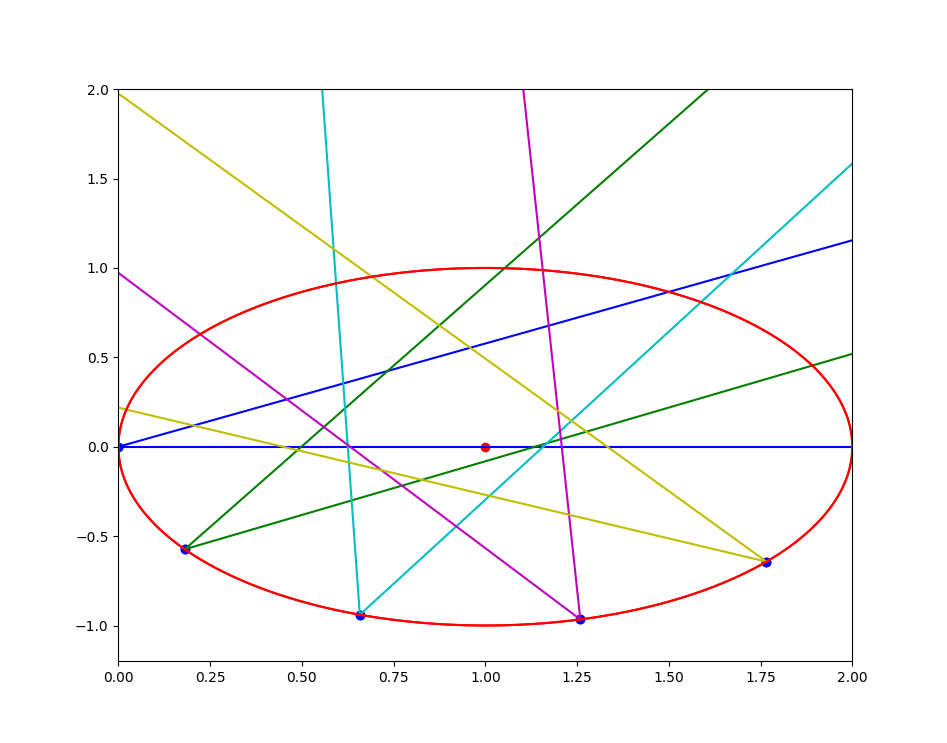
\includegraphics[scale=0.54]{pic1.png} 

如上图所示,五个顶点是在以(1,0)为圆心半径为1的圆上。它们与圆心的角度分别是180, 215, 240, 275, 310度。每个$Z$型的两个边中与$x$轴夹角较小的角度分别是$0,31,62,93,124$ 
\par ~\\

20、令$h(n)=A(n)\alpha +B(n)\gamma _{0}+C(n)\gamma _{1}+D(n)\beta _{0}+E(n)\beta _{1}$,$n=(1b_{m-1}b_{m-2}...b_{2}b_{1}b_{0})_{2}$
\begin{itemize}
	\item 令$\gamma_{0}=\gamma_{1}=0$,跟第16题类似,可以得到:$A(n)=4^m,D(n)=\sum_{i=0}^{m-1}4^{i}(1-b_{i}), E(n)=\sum_{i=0}^{m-1}4^{i}b_{i}$
	\item 令$h(n)=n$可以得到:$\alpha=1,\gamma_{0}=-2,\beta_{0}=0,\gamma_{1}=-2,\beta_{1}=1$,所以$n=A(n)-2B(n)-2C(n)+E(n)$
	\item 令$h(n)=n^{2}$可以得到$n^{2}=A(n)+4C(n)+E(n)$
	\item 由上面两个可以求得$B(n)=\frac{3A(n)+3E(n)-2n-n^{2}}{4},C(n)=\frac{n^{2}-A(n)-E(n)}{4}$
\end{itemize}

\par ~\\
21、如果删除的序列是确定的话,那么可以得到若干个模方程。假设$n=3$: \par
(1)删除的序列是4,5,6,那么有$m$\%6=4, $m$\%5=1, $m$\%4=3,可以看出满足这样的$m$是不存在的,因为$m$\%6=4要求$m$是偶数,而$m$\%4=3要求$m$是奇数。\par
(2)删除的序列是5,4,6,那么有$m$\%6=5, $m$\%5=0, $m$\%4=1,可以看出满足$m=5$可以满足要求,其实所有的$60k+5$都是满足的; \par
这么
算可能有很多种答案。但一定有一个答案是$m=LCM(n+1,n+2,...,2n)$。因为可以从$2n$到$n+1$逆序删掉.这时候要求$m$是$n+1,n+2,..,2n$的最小公倍数。

\end{document}
